\chapter{Configuration TLS/mTLS sur Mosquitto}

\section{Sécurisation du broker MQTT}

\subsection{Architecture de sécurité Mosquitto}

Mosquitto v2.0~\cite{mosquitto_tls} intègre un support natif de TLS via la bibliothèque OpenSSL. La configuration de sécurité retenue repose sur quatre principes fondamentaux :

\begin{enumerate}
  \item \textbf{Désactivation complète du port non chiffré} (1883) -- seul le port 8883 (MQTT/TLS) est exposé.
  \item \textbf{TLS~1.3 obligatoire} -- les versions antérieures sont explicitement interdites.
  \item \textbf{mTLS obligatoire} -- le broker exige un certificat client pour toute connexion.
  \item \textbf{ACL par certificat} -- l'autorisation d'accès aux topics est liée au CN du certificat client.
\end{enumerate}

\subsection{Éléments de configuration principaux}

La configuration du broker Mosquitto repose sur les directives suivantes :

\begin{table}[H]
\centering
\caption{Directives principales de sécurité Mosquitto}
\label{tab:mosquitto_directives}
\begin{tabular}{llp{5.5cm}}
\toprule
\textbf{Directive} & \textbf{Valeur} & \textbf{Description} \\
\midrule
\texttt{listener} & 8883 & Port unique TLS \\
\texttt{cafile} & \texttt{ca-chain.crt} & Chaîne CA de confiance \\
\texttt{certfile} & \texttt{server.crt} & Certificat du serveur \\
\texttt{keyfile} & \texttt{server.key} & Clé privée du serveur \\
\texttt{require\_certificate} & \texttt{true} & mTLS obligatoire \\
\texttt{use\_identity\_as\_username} & \texttt{true} & CN comme identifiant MQTT \\
\texttt{tls\_version} & \texttt{tlsv1.3} & TLS~1.3 strict \\
\texttt{allow\_anonymous} & \texttt{false} & Connexions anonymes interdites \\
\bottomrule
\end{tabular}
\end{table}

La configuration complète du fichier \texttt{mosquitto.conf} est disponible en Annexe~B (section~\ref{sec:config_mosquitto}).

\subsection{Politiques ACL}

Le fichier ACL associe le CN du certificat client aux topics autorisés. Chaque dispositif IoT se voit attribuer un espace de noms dédié : il peut publier sur \texttt{iot/sensors/<device-id>/\#} et s'abonner à \texttt{iot/commands/<device-id>/\#}. Un service de monitoring dispose d'un accès en lecture sur l'ensemble des topics.

Le détail des politiques ACL est fourni en Annexe~B.

\section{Déploiement dans Docker/GNS3}

Le broker Mosquitto est déployé sous forme de conteneur Docker dans l'environnement GNS3. L'image est construite à partir de l'image officielle \texttt{eclipse-mosquitto:2.0}, enrichie des certificats TLS et des fichiers de configuration. Les permissions sur la clé privée du serveur sont restreintes (mode 600) conformément aux bonnes pratiques de sécurité.

Le Dockerfile complet est documenté en Annexe~B.

\section{Validation de la configuration TLS}

\subsection{Tests de connexion}

La validation de la configuration TLS/mTLS s'effectue en deux étapes :

\begin{enumerate}
  \item \textbf{Test négatif} : Une connexion sans certificat client est tentée. Le broker rejette la connexion avec une erreur \texttt{SSL alert handshake failure}, confirmant que le mTLS est bien obligatoire.
  \item \textbf{Test positif} : Une connexion avec un certificat client valide (émis par la CA intermédiaire Vault) est établie avec succès. Le protocole négocié est TLS~1.3, la cipher suite sélectionnée est \texttt{TLS\_AES\_256\_GCM\_SHA384}.
\end{enumerate}

Les commandes de test détaillées sont fournies en Annexe~A.

\subsection{Test fonctionnel MQTT}

Un test \textit{publish/subscribe} est réalisé avec les utilitaires \texttt{mosquitto\_pub} et \texttt{mosquitto\_sub}, en fournissant les certificats mTLS. Ce test valide le fonctionnement complet de la chaîne : authentification mutuelle, routage par topic et réception du message.

\section{Analyse du handshake TLS 1.3}

Le diagramme de séquence de la figure~\ref{fig:tls_handshake} détaille les échanges du handshake TLS~1.3 en mode mTLS, capturé via Wireshark.

\begin{figure}[H]
  \centering
  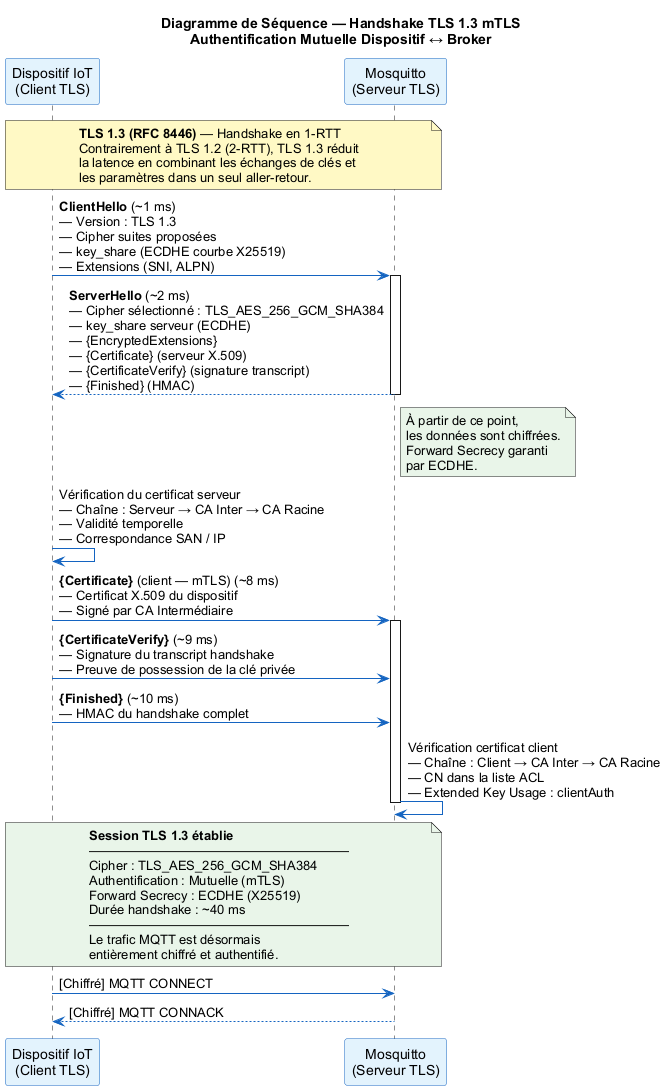
\includegraphics[width=0.7\textwidth]{diagrams/diag-tls-handshake.png}
  \caption{Handshake TLS~1.3 mTLS -- diagramme de séquence détaillé}
  \label{fig:tls_handshake}
\end{figure}

Le tableau~\ref{tab:handshake_tls} présente la décomposition temporelle de chaque étape du handshake.

\begin{table}[H]
\centering
\caption{Analyse temporelle du handshake TLS~1.3 en mTLS}
\label{tab:handshake_tls}
\begin{tabular}{llp{6cm}}
\toprule
\textbf{Étape} & \textbf{Durée} & \textbf{Description} \\
\midrule
ClientHello & < 1~ms & Propose TLS~1.3, cipher suites, \texttt{key\_share} \\
ServerHello & $\sim$2~ms & Sélectionne \texttt{TLS\_AES\_256\_GCM\_SHA384}, renvoie \texttt{key\_share} serveur \\
EncryptedExtensions & $\sim$3~ms & Extensions chiffrées (ALPN, SNI) \\
Certificate (serveur) & $\sim$5~ms & Certificat X.509 du broker \\
CertificateVerify & $\sim$6~ms & Signature du transcript par le serveur \\
Finished (serveur) & $\sim$7~ms & HMAC du handshake \\
Certificate (client) & $\sim$8~ms & Certificat X.509 du dispositif (mTLS) \\
CertificateVerify & $\sim$9~ms & Signature par le dispositif \\
Finished (client) & $\sim$10~ms & Établissement complet de la session \\
\bottomrule
\end{tabular}
\end{table}

\begin{resultbox}[Résultat TLS/mTLS]
Durée totale du handshake TLS~1.3 mTLS : \textbf{$\sim$40~ms} (overhead mesuré expérimentalement).\\
Cipher suite sélectionnée : \texttt{TLS\_AES\_256\_GCM\_SHA384}.\\
Toutes les connexions sans certificat client valide sont rejetées.\\
50 dispositifs connectés simultanément sans dégradation notable.
\end{resultbox}
